
\section{Lightweight Audio Obfuscation}
\label{sec:obfuscation}

\TODO{small overview of both methods}

\TODO{describe data collected from mechanical turk in figure \ref{fig:mturk_survey}}. The first 4 bars correspond to decreasing decimated frequencies. \\ The last four bars correspond to decreasing bit depth of audio.

\afterpage{
    \begin{figure}[H]
    \centering
    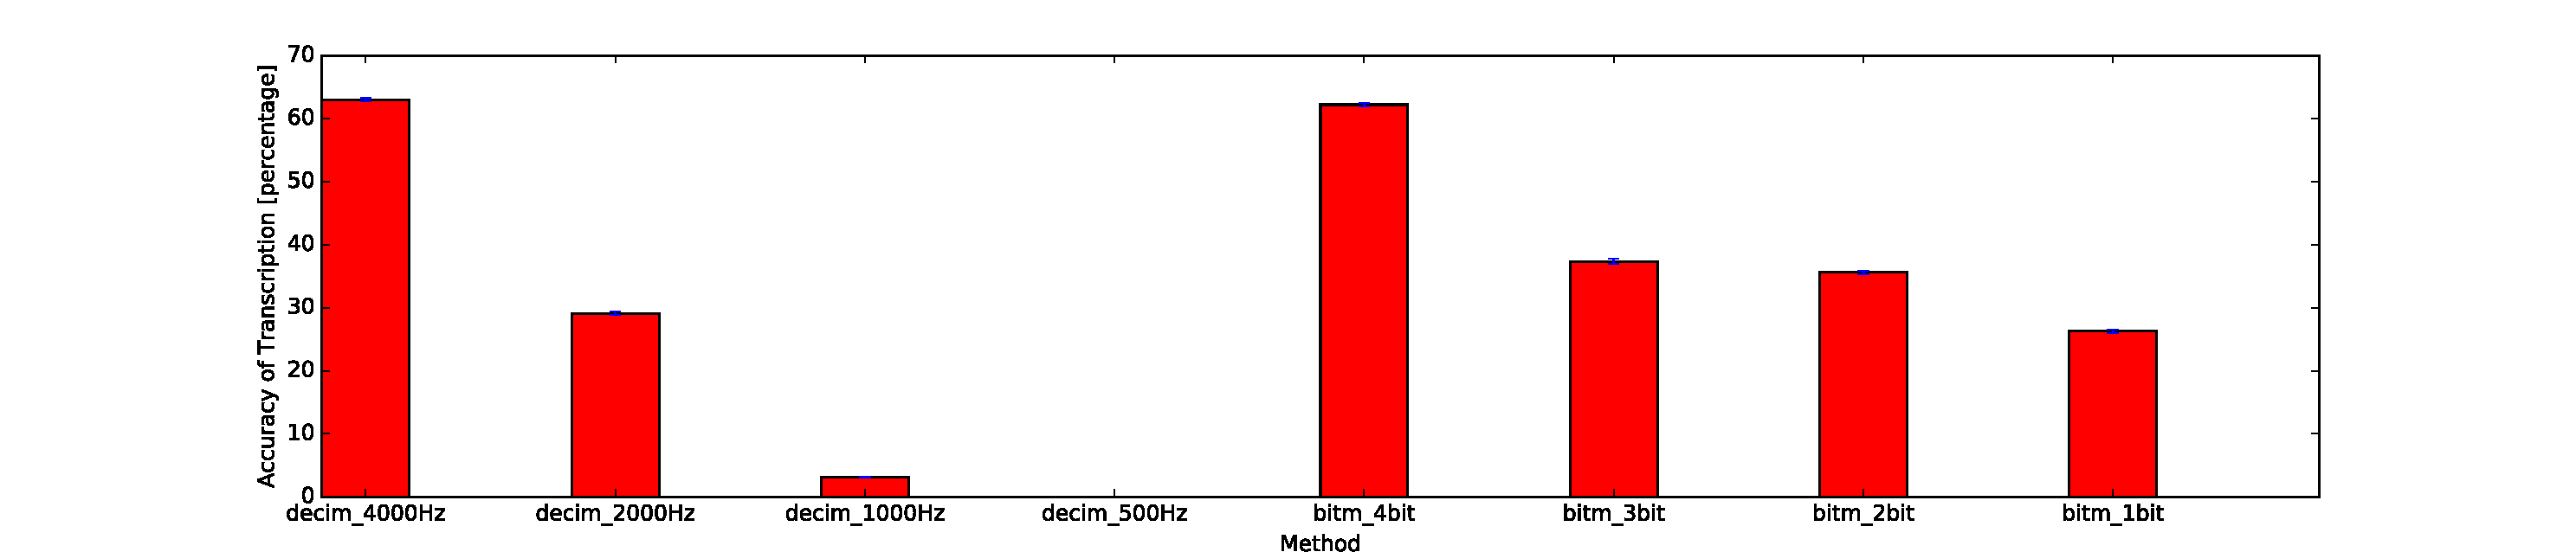
\includegraphics[width=\textwidth]{sound/mturk_survey.pdf}
    \caption{Accuracy of human transcription for different levels of decimation and quantization.}
    \label{fig:mturk_survey}
    \end{figure}
    \begin{table}[H]
    \begin{tabularx}{\textwidth}{l | l | l | l}
    \textbf{Key} & \textbf{Description} & \textbf{Key} & \textbf{Description} \\
    \hline
    decim\_4000 & Decimated to 4 kHZ & bitm\_4bit & 4-bit precision audio \\
    decim\_2000 & Decimated to 2 kHZ & bitm\_3bit & 3-bit precision audio \\
    decim\_1000 & Decimated to 1 kHZ & bitm\_2bit & 2-bit precision audio \\
    decim\_500 & Decimated to 500 HZ & bitm\_1bit & 1-bit precision audio \\
    \end{tabularx}
    \caption{Key for X-axis in Figure \ref{fig:mturk_survey}: \nameref{fig:mturk_survey}}
    \label{tab:key_mturk_survey}
    \end{table}
}

\subsection{Decimation: Removing time fidelity}

If the audio stream is recorded at 16kHz, we decimate the audio stream to a much lower sampling frequency.
 With this operation, the intelligibility of speech rapidly decreases with the amount of decimation.
 However, this also significantly decreases keyword spotting performance.

\TODO{ some raw data vs subsampled data? and the FFT for both to visualize information loss?}

\TODO{figure showing the performance decline of CMUSphinx, Google Speech Recog. with subsampled audio data}

\TODO{discuss the entropy and information content after this operation with respect to the raw audio}

\TODO{use differential privacy to discuss how adding controlled noise to this can prevent an attacker from understanding sensitive information.}


\subsection{Bit Depth: Removing amplitude fidelity}

If the audio stream is recorded at a 16-bit depth, we quantize the audio stream to a much lower bit depth to reduce the information content.
 Surprisingly, we find that, even at the lowest possible 1-bit depth, the speech content can be easily understood by humans (Figure \ref{fig:mturk_survey}).

\TODO{discuss: the loss of information with quantization? not so much}

\TODO{discuss the entropy and information content after this operation with respect to the raw audio}

\TODO{use differential privacy to discuss how adding controlled noise to this can prevent an attacker from understanding sensitive information.}

\subsection{Obfuscating audio using hamming weights}

If we consider each audio sample as one "sample bit", then we can compute the hamming weight of $n$ sample bits.
 This is done by concatenating the sample bit strings and counting the total number of "1"s in the $n$-sample bit string.

\TODO{discuss the entropy and information content after this operation with respect to the raw audio}

\TODO{use differential privacy to discuss how adding controlled noise to this can prevent an attacker from understanding sensitive information.}

\TODO{repeat the two analyses above applying the same hamming weight technique to both decimated audio and low bit-depth audio}

\subsection{Adding keywords to the dictionary}

\TODO{how would adding more keywords affect the privacy vs utility?}

\TODO{can we say if we add keywords with certain characteristics the algorithm will still be fine?}
